\chapter{Dynamic Strategy with Transformers}
\label{chapter:dynamic}

\begin{chapabstract}
    Continual models aim to learn an ever-growing number of tasks. Dynamic architectures expand
    their parameters to tackle this increasing complexity. However,
    existing approaches often require a task identifier at test-time, need complex tuning to balance
    the growing number of parameters, and barely share any information across tasks. As a result,
    they struggle to scale to a large number of tasks without significant overhead.\\
    In this chapter, we propose a transformer architecture based on a dedicated encoder/decoder
    framework. Critically, the encoder and decoder are shared among all tasks. Through a dynamic
    expansion of special tokens, we specialize each forward of our decoder network on a task
    distribution. Our strategy scales to a large number of tasks while having negligible memory and
    time overheads due to strict control of the expansion of the parameters. Moreover, as a result,
    this efficient strategy doesn't need any hyperparameter tuning to control the network's
    expansion.\\
    We evaluate our model on multiple datasets and show the interest of our parameter expansion strategy,
    striking the right balance between performance and overhead. We also extensively ablate our
    model to highlight each component contribution.

    \begin{itemize}
        \item \fullcite{douillard2021dytox}
    \end{itemize}

\end{chapabstract}
\newpage

\minitoc
\chapterwithfigures{\nameref*{chapter:dynamic}} \chapterwithtables{\nameref*{chapter:dynamic}}

\ifthenelse{\boolean{skipDyna}}{\endinput}{}


\section{Introduction}
\label{sec:dytox_intro}


Recent works expand the network architectures or re-arrange their internal structures using dynamic
strategies (see \autoref{sec:related_structural}). Unfortunately at test-time, they require to know
the task to which the test sample belongs --- in order to know which parameters should be used. More
recently, DER \citep{yan2021der} and Simple-DER \citep{li2021preserve} discarded the need for this
task identifier by learning a single classifier on the concatenation of all produced embeddings by
different subsets of parameters. Yet, these strategies induce an important memory overhead when
tackling a large number of tasks, and thus need complex pruning as post-processing.

To improve the ease of use of continual learning frameworks for real-world applications, we aim to
design a dynamically expandable representation (almost) ``for free'' by having the three following
properties:

\begin{enumerate}
    \item \textbf{limited memory overhead} as the number of tasks grows,
    \item \textbf{limited time overhead} at test time,
    \item \textbf{no setting-specific hyperparameters} for improved robustness when faced to an unknown
          (potentially large) number of tasks.
\end{enumerate}

%\#1 \textbf{limited memory overhead} as the number of tasks grows, \#2 \textbf{limited
%    time overhead} at test time and \#3 \textbf{no setting-specific hyperparameters} for improved
%robustness when faced to an unknown (potentially large) number of tasks.

To this end, we leverage the computer vision transformers (refer to \autoref{sec:related_cv}).
Transformers \citep{vaswani2017transformer} offer a very interesting framework to satisfy the
previously mentioned constraints. Indeed, we build upon this architecture to design a
\textbf{encoder/decoder strategy}: the encoder layers are shared among all members of our dynamic
network; the unique decoder layer is also shared, but its forward pass is specialized by a
\textbf{task-specific learned token} to produce task-specific embeddings. Thus, the memory growth of
the dynamic network is extremely limited: only a 384d vector per task, validating property \#1.
Moreover, this requires no hyperparameter tuning (property \#3). Finally, the decoder is explicitly
designed to be computationally lightweight (satisfying property \#2). We nicknamed our framework,
DyTox, for \textbf{DYnamic TOken eXpansion}.

Our strategy is robust to different settings, and can easily scale to a large number of tasks with
minimal time and memory overheads. In particular, we validate the efficiency of our approach on
CIFAR100, ImageNet100, and ImageNet1000 for multiple settings. We also perform ablations confirming
the soundness of our dynamic strategy. In this chapter, we focus on continual dynamic networks
(refer to \autoref{sec:related_structural}) that expand their parameters coupled with rehearsal
learning (\autoref{sec:related_rehearsal}). Moreover, to satisfy our desiderata listed previously,
we base our framework on the recent Transformer architecture (see \autoref{sec:related_cv}).

\paragraph{Positioning with respect to PODNet} Note that while our methods PODNet
(\autoref{sec:podnet}) and DyTox (presented in this chapter) are both designed for class-incremental
image classification, they differ in terms of both objective and benchmark: PODNet aims to constrain
the features drift to reduce forgetting, while DyTox conditions features to a particular task.
Moreover, PODNet, a metric-based model, requires a larger initial task size to perform well.
Therefore, PODNet was evaluated when half of the dataset's classes are seen in the first step. On
the other hand, DyTox is considered here in the setting of \citet{yan2021der} where all steps,
including the first one, bring an equal number of new classes.

\section{DyTox transformer model}
\label{sec:dytox_model}

\begin{figure*}
    \centering
    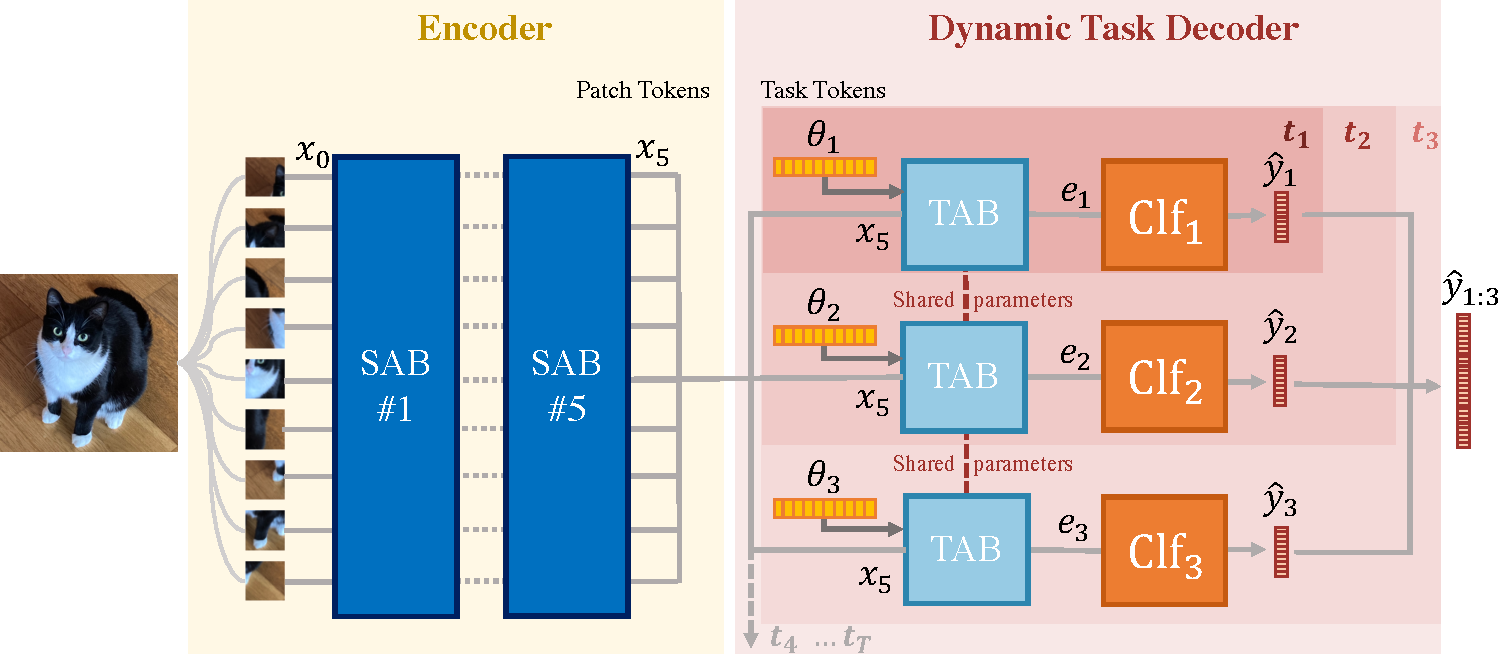
\includegraphics[width=0.95\textwidth]{images/dytox/dytox.pdf}
    \caption{\textbf{DyTox transformer model}. An image is first split into multiple patches,
    embedded with a linear projection. The resulting patch tokens are processed by 5 successive
    Self-Attention Blocks (SAB) (\autoref{sec:related_cv}). For each task ($t = 1\dots T$), the processed
    patch tokens are then given to the Task-Attention Block (TAB) (\autoref{sec:dytox_tab}): each forward
    through the TAB is modified by a different task-specialized token $\theta_t\, \text{for}\, t \in
        \{1 \dots T\}$ (\autoref{sec:dytox_ensembling_tab}). The $T$ final embeddings are finally given
    separately to independent classifiers $\text{Clf}_t$ each predicting their task's classes $C^t$.
    All $|C^{1:T}|$ logits are activated with a sigmoid. For example, at task $t=3$, one forward is
    done through the SABs and three task-specific forwards through the unique TAB.}
    \label{fig:dytox_model}
\end{figure*}

\label{sec:dytox_problem}

%Our goal is to learn a unified model that will classify an increasingly growing number of classes,
%introduced in a fixed amount of steps $T$. At a given step $t \in \{1 \dots T\}$, the model is
%exposed to new data belonging to new classes. Specifically, it learns from samples $\{(x_i^t,
%      y_i^t)\}_{i}$, where $x_i^t$ is the $i$-th image of this task $t$ and $y_i^t$ is the associated
%label within the label set $\mcC^t$. All task label sets are exclusive: $\mcC^0 \cap \mcC^1 \dots
%      \mcC^T = \emptyset$. The main challenge is that the data are fully available only temporarily:
%following most previous works, only a few samples from previous tasks $\{1 \dots t-1\}$ are
%available for training at step $t$ as rehearsing data. Yet, the model should remain able to classify
%test data coming from all seen classes $\mcC^{1:t}$. A table of notations is provided in the
%supplementary materials.

We evaluate our framework in the \acf{CIL} setting (\autoref{sec:related_continual}) where each task
brings an equal number of new classes. We also use rehearsal learning
(\autoref{sec:related_rehearsal}). The \autoref{fig:dytox_model} displays our DyTox framework, which
is made of several components (SAB, TAB, and Task Tokens) that we describe in the following
sections.

\subsection{Background}
\label{sec:dytox_vit}

The vision transformer \citep{dosovitskiy2020vit} has three main components: the patch tokenizer, the
encoder made of Self-Attention Blocks (SABs), and the classifier. We described in the related work
(\autoref{sec:related_cv}) the general architecture. A SAB is depicted in \autoref{fig:dytox_sab}.

\begin{figure}
    \centering
    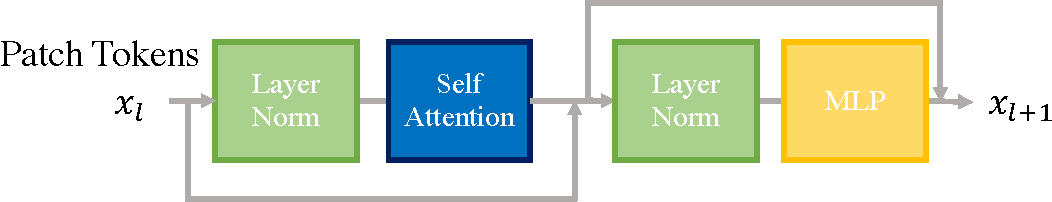
\includegraphics[width=1\textwidth]{images/dytox/sab.pdf}
    \caption{\textbf{The Self-Attention Block (SAB)} combines a Self-Attention (SA), two Layer
        Norms, and one MLP with a single hidden layer. As in a ResNet, two shortcuts are used with
        element-wise addition.}
    %\vspace{-2em}
    \label{fig:dytox_sab}
\end{figure}

Importantly, recall that in the original vision transformer ViT \citep{dosovitskiy2020vit}, a learned
vector called the ``\textit{class token}'' is appended to the patch tokens after the tokenizer. This
special class token, when processed after all the SABs, is given to a linear classifier with a
softmax activation to predict the final probabilities. However, more recent works, as CaiT
\citep{touvron2021cait}, propose instead to introduce the class token only at the ultimate or
penultimate SAB to improve classification performance.

\subsection{Task-Attention Block (TAB)}
\label{sec:dytox_tab}

Contrary to previous transformer architectures, we don't have a class token, but rather what we
nicknamed ``\textbf{task tokens}''; the learned token of the $i^{th}$ task is denoted $\theta_i$.
This special token will only be added at the last block. To exploit this task token, we define a new
attention layer, that we call the Task-Attention. It first concatenates the patch tokens $x_L$
produced by the ultimate SAB with a task token $\theta_i$:
%
\begin{equation}
    z_i = [\theta_i, x_L] \, \in \mathbb{R}^{(\mathbb{N} + 1) \times \mathbb{D}}\,.
    \label{eq:dytox_concat_cls_token}
\end{equation}
%
This is then given to the Task-Attention (TA), inspired by the Class-Attention of Touvron et al.
\citep{touvron2021cait}:
%
\begin{equation}
    \begin{aligned}
        Q_i & =W_{q} \theta_i\,,                                                      \\
        K_i & =W_{k} z_i\,,                                                           \\
        V_i & =W_{v} z_i\,,                                                           \\
        A_i & =\operatorname{Softmax}\left(Q_i \cdot K_i^{T} / \sqrt{d / h}\right)\,, \\
        O_i & = W_{o} A_i V_i+b_{o} \, \in \mathbb{R}^{1 \times \mathbb{D}}\,,
    \end{aligned}
    \label{eq:dytox_ca_layer}
\end{equation}
%
with $d$ being the embedding dimension, and $h$ the number of attention heads
\citep{vaswani2017transformer}. Contrary to the classical Self-Attention, the Task-Attention defines
its query ($Q_i$) only from the task-token $\theta_i$ without using the patch tokens $x_L$. The
Task-Attention Block (TAB) is then a variation of the SAB where the attention is a Task-Attention
(TA):
\begin{equation}
    \begin{aligned}
        c^{\prime}       & =c+\operatorname{TA}\left(\operatorname{Norm}_1\left(z\right)\right)\,,                    \\
        c^{\prime\prime} & =c^{\prime}+\operatorname{MLP}\left(\operatorname{Norm}_2\left(c^{\prime}\right)\right)\,.
    \end{aligned}
    \label{eq:dytox_ca_block}
\end{equation}
Overall, our new architecture can be summarized by the repetition of SA Blocks
$\{\operatorname{SAB}_l\}_{l=1}^{L}$ (defined in \autoref{eq:related_sa}) ended by a single TA Block
$\operatorname{TAB}$ (defined in \autoref{eq:dytox_ca_block}):
%
\begin{equation}
    e_i = \operatorname{TAB} \circ\, ([\theta_i,\, \operatorname{SAB}_{l=L} \circ\, ... \operatorname{SAB}_{l=1}(x_0)]) \in \mathbb{R}^D\,.
    \label{eq:dytox_cab_sab}
\end{equation}
%
The final embedding $e_i$ is fed to a classifier $\operatorname{clf}$ made of a
$\operatorname{Norm}_c$ and a linear projection parametrized by $\{W_c, b_c\}$:
%
\begin{equation}
    \tilde{y}_i = \operatorname{Clf}(e_i) = W_c \operatorname{Norm}_c(e_i) + b_c\,.
\end{equation}

\subsection{Dynamic task token expansion}
\label{sec:dytox_ensembling_tab}
We defined in the previous section our base network, made of a succession of SABs and ended by a
single TAB. As detailed, the TAB has two inputs: the patch tokens $x_L$ extracted from the image and
a learned task-token $\theta_i$. We'll now detail how our framework evolves in a continual situation
at each new step.

During the first step, there is only one task token $\theta_1$. At each new step, we propose to
expand our parameter space by creating a new task token while keeping the previous ones. Thus, after
$t$ steps, we have $t$ task tokens ($\theta_i\,\text{for}\, i\in \{1 \dots t\}$). Given an image $x$
--- belonging to any of the seen tasks $\{1\dots \, t\}$ --- our model tokenizes it into $x_0$, and
processes it through the multiple SABs: this outputs the patch tokens $x_L$. Finally, our framework
does as many forward passes through the TAB as there are tasks: critically, each TAB forward passes
is executed with a different task token $\theta_i$, resulting in different task-specific forwards,
each producing the task-specific embeddings $e_i$ (see \autoref{fig:dytox_model}):
%
\begin{equation}
    \begin{aligned}
         & e_1 = \operatorname{TAB}([\theta_1, x_L])\,, \\
         & e_2 = \operatorname{TAB}([\theta_2, x_L])\,, \\
         & \dots                                        \\
         & e_t = \operatorname{TAB}([\theta_t, x_L])\,. \\
    \end{aligned}
    \label{eq:dytox_multiple_tab}
\end{equation}
%
Rather than concatenating all embeddings $\{e_1, e_2, \dots, e_t\}$ together and feeding them to one
classifier, we leverage \textbf{task-specific classifiers}. Each classifier $\operatorname{clf}_i$
is made of a $\operatorname{Norm}_i$ and a linear projection parametrized by $\{W_i, b_i\}$, with
$W_i \in \mathbb{R}^{\mcC^i \times D}$ and $b \in \mathbb{R}^{\mcC^i}$. It takes as input its
task-specific embedding $e_i$ and returns:
%
\begin{equation}
    \hat{y}_i = \operatorname{Clf}_i(e_i) = \sigma(W_i \operatorname{Norm}_i e_i + b_i)\,,
    \label{eq:dytox_ind_clf}
\end{equation}
%
the predictions for the classes $y_i \in \mcC^i$, where $\sigma(x) = \nicefrac{1}{(1 + e^{-x})}$ is
the sigmoid activation. In comparison with the softmax activation, the element-wise sigmoid
activation reduces the overconfidence in recent classes. Consequently, the model is better
calibrated, which is an important attribute of continual model
\citep{belouadah2019il2m,wu2019bias_correction,zhao2020weightalignement}. The loss is the
binary-cross entropy. The independent classifiers paradigm coupled with the sigmoid activation and
binary cross-entropy loss exclude explicitly a late fusion \citep{ramachandram2017multimodalreview}
of the task embeddings resulting in more \textbf{specialized classifiers}.

\paragraph{The overall structure of the DyTox strategy} is illustrated in \autoref{fig:dytox_model}.
We also show in \autoref{algo:dytox_tab_ensemble_1-1_bce} the pseudo-code of a forward pass at test-time
after having learned the task $t$. Critically, the test image can belong to any of the previously
seen tasks $\{1 \,\dots \, t\}$. Our dynamic task token expansion is more efficient than a naive
parameter expansion that would create a new copy of the whole network for each new task. (1) Our
expansion is limited to a new task token per new task, which is only $d=384$ new parameters. This is
small compared to the total model size ($\approx$ 11 million parameters). The \textbf{memory
    overhead is thus almost null}. (2) The computationally intensive blocks (\textit{i.e.}, the SABs)
are executed only once despite learning multiple tasks. In contrast, the TAB has as many forwards as
there are tasks. Though, this induces minimal overhead because the \textbf{Task-Attention has a
    linear complexity w.r.t the number of patches} while the Self-Attention is quadratic. Therefore, the
time overhead is sub-linear. We quantitatively show this in \autoref{sec:dytox_exp}.

\begin{algorithm}[tb]
    \caption{DyTox's forward pass at step $t$}
    \label{algo:dytox_tab_ensemble_1-1_bce}
    \hspace*{\algorithmicindent} \textbf{Input:} $x_0$ (initial patch tokens), $y$ ( ground-truth
    labels) \\
    \hspace*{\algorithmicindent} \textbf{Output:} $\hat{y}_{1:t}$ (predictions for all classes of
    $\mcC^{1:t}$)
    \begin{algorithmic}[1]
        % \Require $x_0$ (initial patch tokens), $y$ ( ground-truth labels)
        \State $x_L \gets \operatorname{SAB}_{l=L} \circ ... \operatorname{SAB}_{l=1}(x_0)$
        \Comment{\autoref{sec:dytox_vit}}

        \For{\texttt{$i \gets 1$; $i \leq t$; $i{+}{+}$}} \State $e_i \gets \operatorname{TAB}([\theta_i,
                x_L])$ \Comment{\autoref{sec:dytox_tab}} \State $\hat{y}_i \gets \operatorname{Clf}_i(e_i)$
        \Comment{\autoref{sec:dytox_ensembling_tab}} \EndFor

        \State $\hat{y}_{1:t} \gets [\hat{y}_1,\, \dots,\, \hat{y}_{t}]$
    \end{algorithmic}
\end{algorithm}

%\vspace{-1em}
\paragraph{Context} The current transformer paradigm starting from BERT \citep{devlin2018bert} and
continuing with ViT \citep{dosovitskiy2020vit} is based on a encoder+classifier structure.
Differently, our dynamic framework strays is a resurgence of the encoder/decoder structure of the
original transformer \citep{vaswani2017transformer}: the encoder is shared (both in memory and
execution) for all outputs. The decoder parameters are also shared, but its execution is
task-specific with each task token, with each forward akin to a task-specific expert chosen from a
mixture of experts \citep{masoudnia2014mixture}. Moreover, multi-tasks text-based transformers have
natural language tokens as an indicator of a task \citep{raffel2019t5} (\eg "summarize the
following text"), in our context of vision we used our defined task tokens as indicators.

\label{sec:dytox_training}

%\vspace{-0.5em}
\paragraph{Losses} Our model is trained with three losses: (1) the classification loss
$\mathcal{L_\text{clf}}$, a binary-cross entropy, (2) a knowledge distillation
\citep{hinton2015knowledge_distillation} $\mathcal{L_\text{kd}}$ applied on the probabilities, and
(3) the divergence loss $\mathcal{L_\text{div}}$. The distillation loss helps to reduce forgetting.
It is arguably quite naive, and more complex distillation losses
\citep{selvaraju2017gradcam,hou2019ucir} could further improve results. The
divergence loss, inspired from the ``auxiliary classifier'' of DER \citep{yan2021der}, uses the
current last task's embedding $e_t$ to predict ($|\mcC^t| + 1$) probabilities: the current last
task's classes $\mcC^t$ and an extra class representing all previous classes that can be encountered
via rehearsal. This classifier is discarded at test-time and encourages a better diversity among
task tokens. The total loss is:
%
\begin{equation}
    \mathcal{L} = (1 - \alpha) \mathcal{L_\text{clf}} + \alpha \mathcal{L_\text{kd}} + \lambda \mathcal{L_\text{div}}\,,
    \label{eq:dytox_final_loss}
\end{equation}
%
with $\lambda$ a hyperparameter set to $0.1$ for \textbf{all} experiments. $\alpha$ correspond to
the fraction of the number of old classes over the number of new classes
$\frac{|C^{1:t-1}|}{|C^{1:t}|}$ as done by \citet{zhao2020weightalignement}. Therefore, $\alpha$ is
automatically set; this removes the need to finely tune this hyperparameter.

\subsection{Improved Continual Training Procedure}

We nicknamed our model described previously DyTox. In this section, we propose two modifications
of the training procedure aimed at improving the continual performance.

\paragraph{DyTox+} We introduce a new efficient training procedure for continual learning. Using MixUp
\citep{hingyi2018mixup}, we linearly interpolate new samples with existing samples. The interpolation
factor $\lambda \sim \operatorname{Beta}(\alpha, \alpha)$ is sampled with $\alpha=0.8$: the pixels
of two images are mixed ($x = \lambda x_1 + (1 - \lambda) x_2$) as their labels ($y = \lambda y_1 +
    (1 - \lambda) y_2$). MixUp was shown to have two main effects: (1) it diversifies the training
images and thus enlarges the training distribution on the vicinity of each training sample
\citep{chapelle2001vicinalrisk} and (2) it improves the network calibration
\citep{guo2017miscalibration,thulasidasan2019mixupcalibration}, reducing the overconfidence in recent
classes. Thus, MixUp has shared motivation with the sigmoid activation. When DyTox is combined with
this MixUp procedure, nicknamed as DyTox+, the forgetting is significantly reduced as shown in
experiments.

\paragraph{DyTox++} We nicknamed DyTox+ our model when combined with a novel continual procedure
based on MixUp \citep{hingyi2018mixup}. We now refine DyTox+ into DyTox++ by adding a new component
during the training: the Sharpness-Aware Minimizer (SAM) \citep{foret2020sam}. Indeed, \textbf{aiming
    for wider minima} is particularly important in continual learning
\citep{kirkpatrick2017ewc,verwimp2021rehearsalrevealed}. This is because sharp task-specific minima
lead to over-specialization to a particular task and consequently to a forgetting of all other
tasks. Weights constraints as EWC \citep{kirkpatrick2017ewc} or second-order optimization
\citep{lee2020kroneckercontinual} have similar motivations. SAM estimates the worst closest
parameters during a first forward/backward pass, and then optimizes the loss w.r.t. to them during a
second forward/pass. In consequence, DyTox++ optimizes the loss not w.r.t. the current parameters
but w.r.t. a region of possible parameters leading to wide local minima that span across multiple
tasks. In practice, we used the Adaptive SAM (ASAM) \citep{kwon2021asam}, an extension of SAM that is
more robust to hyperparameters.


\section{Experiments}
\label{sec:dytox_exp}

\subsection{Benchmarks \& implementation}

\paragraph{Benchmarks \& Metrics} We evaluate our model on CIFAR100 \citep{krizhevskycifar100},
ImageNet100 and ImageNet1000 \citep{deng2009imagenet} (descriptions in the supplementary materials)
under different settings.
%where for each the number of new classes seen per step is different.
The standard continual scenario in ImageNet has 10 steps: thus we add 10 new classes per step in
ImageNet100, and 100 new classes per step in ImageNet1000. In CIFAR100, we compare performances on
10 steps (10 new classes per step), 20 steps (5 new classes per step), and 50 steps (2 new classes
per step). In addition to the top-1 accuracy, we also compare the top-5 accuracy on ImageNet. We
report the ``\textit{Avg}'' accuracy which is the average of the accuracies after each step as
defined by \citep{rebuffi2017icarl}. We also report the final accuracy after the last step
(``\textit{Last}''). Finally, in our tables, ``\textit{\#P}'' denotes the parameters count in
million after the final step.

\begin{table}[t]
    \centering
    \begin{tabular}{@{}l|cc@{}}
        \hline
        Hyperparameter      & CIFAR                   & ImageNet \Tstrut\Bstrut \\
        \hline
        \# SAB              & \multicolumn{2}{c}{5}                             \\
        \# CAB              & \multicolumn{2}{c}{1}                             \\
        \# Attentions Heads & \multicolumn{2}{c}{12}                            \\
        Embed Dim           & \multicolumn{2}{c}{384}                           \\
        Input Size          & 32                      & 224                     \\
        Patch Size          & 4                       & 16                      \\
        \hline
    \end{tabular}
    \caption{\textbf{DyTox's architectures} for CIFAR and ImageNet. The only difference between the
        two architectures is the patch size, as the image sizes vary between datasets.}
    \label{tab:dytox_archi}
\end{table}


\begin{table*}[t]
    \centering
    %	\hspace{mm}
    \begin{tabular}{l|ccccc|ccccc}
        \toprule[0.3mm]
                                                                 & \multicolumn{5}{c|}{ImageNet100 10 steps} & \multicolumn{5}{c}{ImageNet1000 10 steps}                                                                                                                                                                                                                                                           \\
        \cmidrule{2-11}
                                                                 & \multirow{2}{*}{\textbf{$\#$P}}           & \multicolumn{2}{c}{\textbf{top-1}}        & \multicolumn{2}{c|}{\textbf{top-5}} & \multirow{2}{*}{\textbf{$\#$P}} & \multicolumn{2}{c}{\textbf{top-1}} & \multicolumn{2}{c}{\textbf{top-5}}                                                                                                         \\
        \cmidrule{3-6}
        \cmidrule{8-11}
        \textbf{Methods}                                         &                                           & \textbf{Avg}                              & \textbf{Last}                       & \textbf{Avg}                    & \textbf{Last}                      &                                    & \textbf{Avg}            & \textbf{Last}           & \textbf{Avg}            & \textbf{Last}           \\
        \hline
        ResNet18 joint                                           & $11.22$                                   & -                                         & -                                   & -                               & $95.10$                            & $11.68$                            & -                       & -                       & -                       & $89.27$                 \\
        Transf. joint                                            & 11.00                                     & -                                         & 79.12                               & -                               & 93.48                              & 11.35                              & -                       & 73.58                   & -                       & 90.60                   \\
        \midrule
        LwF-MC \cite{li2018lwf,rebuffi2017icarl}                 & 11.2                                      & -                                         & -                                   & 80.79                           & 66.43                              & 11.2                               & -                       & -                       & 48.45                   & 25.06                   \\
        \textit{E2E} \cite{castro2018end_to_end_inc_learn}       & 11.22                                     & -                                         & -                                   & 89.92                           & 80.29                              & 11.68                              & -                       & -                       & 72.09                   & 52.29                   \\
        \textit{Simple-DER} \cite{li2021preserve}                & -                                         & -                                         & -                                   & -                               & -                                  & 28.00                              & 66.63                   & 59.24                   & 85.62                   & 80.76                   \\
        iCaRL \cite{rebuffi2017icarl}                            & $11.22$                                   & -                                         & -                                   & $83.60$                         & $63.80$                            & $11.68$                            & $38.40$                 & $22.70$                 & $63.70$                 & $44.00$                 \\
        BiC \cite{hou2019ucir}                                   & $11.22$                                   & -                                         & -                                   & $90.60$                         & $84.40$                            & $11.68$                            & -                       & -                       & $84.00$                 & $73.20$                 \\
        WA \cite{zhao2020weightalignement}                       & $11.22$                                   & -                                         & -                                   & $91.00$                         & $84.10$                            & $11.68$                            & $65.67$                 & $55.60$                 & $86.60$                 & $81.10$                 \\
        RPSNet \cite{rajasegaran2019rpsnet}                      &                                           & -                                         & -                                   & $87.90$                         & $74.00$                            & -                                  & -                       & -                       & -                       & -                       \\
        DER w/o P \cite{yan2021der}                              & 112.27                                    & \textbf{77.18}                            & 66.70                               & \textbf{93.23}                  & 87.52                              & 116.89                             & 68.84                   & 60.16                   & 88.17                   & 82.86                   \\ % no pruning
        \textcolor{gray}{$\text{DER}^\dagger$} \cite{yan2021der} & \textcolor{gray}{-}                       & \textcolor{gray}{76.12}                   & \textcolor{gray}{66.06}             & \textcolor{gray}{92.79}         & \textcolor{gray}{88.38}            & \textcolor{gray}{-}                & \textcolor{gray}{66.73} & \textcolor{gray}{58.62} & \textcolor{gray}{87.08} & \textcolor{gray}{81.89} \\
        \hline
        DyTox                                                    & 11.01                                     & \textbf{77.15}                            & \textbf{69.10}                      & 92.04                           & \textbf{87.98}                     & 11.36                              & \textbf{71.29}          & \textbf{63.34}          & \textbf{88.59}          & \textbf{84.49}          \\
        \hline
    \end{tabular}
    \caption{\textbf{Results on ImageNet-100  and ImageNet-1000 datasets}, learned with 10 steps of
        respectively 10 and 100 new classes. E2E \cite{castro2018end_to_end_inc_learn} and Simple-DER
        \cite{li2021preserve} results come from their respective papers, and used a different class
        ordering. Other results come from \cite{yan2021der}. The $\dagger$ symbol means that
        \cite{yan2021der} needed setting-sensitive hyperparameters. Moreover, its reported parameters
        count was an average over all steps (\cite{yan2021der} reported 14.52M on ImageNet1000): the
        final parameters count (necessarily higher) was not available.}
    \label{tab:dytox_imagenet}
\end{table*}

\begin{table}[t]
    \centering
    %\resizebox{\textwidth}{!}{%
    \begin{tabular}{l|ccccc}
        \hline
        \multirow{2}{*}{\textbf{Methods}}                & \multirow{2}{*}{\textbf{$\#$P}} & \multicolumn{2}{c}{\textbf{top-1}} & \multicolumn{2}{c}{\textbf{top-5}}                                   \\
                                                         &                                 & \textbf{Avg}                       & \textbf{Last}                      & \textbf{Avg}   & \textbf{Last}  \\
        \hline
        ResNet18 joint                                   & $11.22$                         & -                                  & -                                  & -              & $95.1$         \\
        Transf. joint                                    & 11.00                           & -                                  & 79.12                              & -              & 93.48          \\
        \hline
        WA \scriptsize{\citep{zhao2020weightalignement}} & $11.22$                         & -                                  & -                                  & $91.00$        & $84.10$        \\
        DER w/o P \scriptsize{\citep{yan2021der}}        & 112.27                          & 77.18                              & 66.70                              & 93.23          & 87.52          \\
        \hline
        DyTox                                            & 11.01                           & 77.15                              & 69.10                              & 92.04          & 87.98          \\
        DyTox+                                           & 11.01                           & 79.22                              & 69.06                              & 93.72          & 88.82          \\
        DyTox++                                          & 11.01                           & \textbf{80.76}                     & \textbf{72.46}                     & \textbf{94.40} & \textbf{90.10} \\
        \hline
    \end{tabular}
    %}
    \caption{\textbf{Results on ImageNet-100} with 10 steps of 10 new classes each. WA and DER w/o P
        results are reported from \cite{yan2021der}. DyTox+ uses MixUp in addition of the DyTox
        strategy, DyTox++ further adds a sharpness-aware minimizer.}
    \label{tab:dytox_imagenet_pp}
\end{table}




\paragraph{Implementation details} As highlighted in \autoref{tab:dytox_archi}, our network has the same
structure across all tasks. Specifically, we use 5 Self-Attention Blocks (SABs), 1 Task-Attention
Block (TAB). All 6 have an embedding dimension of 384 and 12 attention heads. We designed this
shallow transformer to have a comparable parameters count to other baselines, but also made it wider
than usual "tiny" models \citep{dosovitskiy2020vit,touvron2021deit,touvron2021cait}. We tuned all
hyperparameters for CIFAR100 with 10 steps on a validation set made of 10\% of the training set, and
then kept them fixed for all other settings, ImageNet included. The only difference between the two
datasets is that ImageNet images are larger; thus the patch size is larger, and overall the base
transformer has slightly more parameters on ImageNet than on CIFAR (11.00M \vs 10.72M) because of a
bigger positional embedding. We use the attention with spatial prior (introduced by ConViT
\citep{dascoli2021convit}) for all SABs, which allows training transformers on a small dataset (like
CIFAR) without pretraining on large datasets or complex regularizations. Following previous works
\citep{rebuffi2017icarl,yan2021der}, we use for all models (baselines included) 2,000 images of
rehearsal memory for CIFAR100 and ImageNet100, and 20,000 images for ImageNet1000. The Continuum
library \citep{douillardlesort2021continuum} provides the implementations of the continual
scenarios. Our network implementation is based on the DeiT \citep{touvron2021deit} code base, which
itself extensively uses the timm library \citep{wightman2019timm}. The code is released
publicly\footnote{\footnotesize{\url{https://github.com/arthurdouillard/dytox}.}}. The full
implementation details are in the appendix (\autoref{sec:appendix_dytox}).


\begin{figure}
    \centering
    \begin{subfigure}{.5\textwidth}
        \centering
        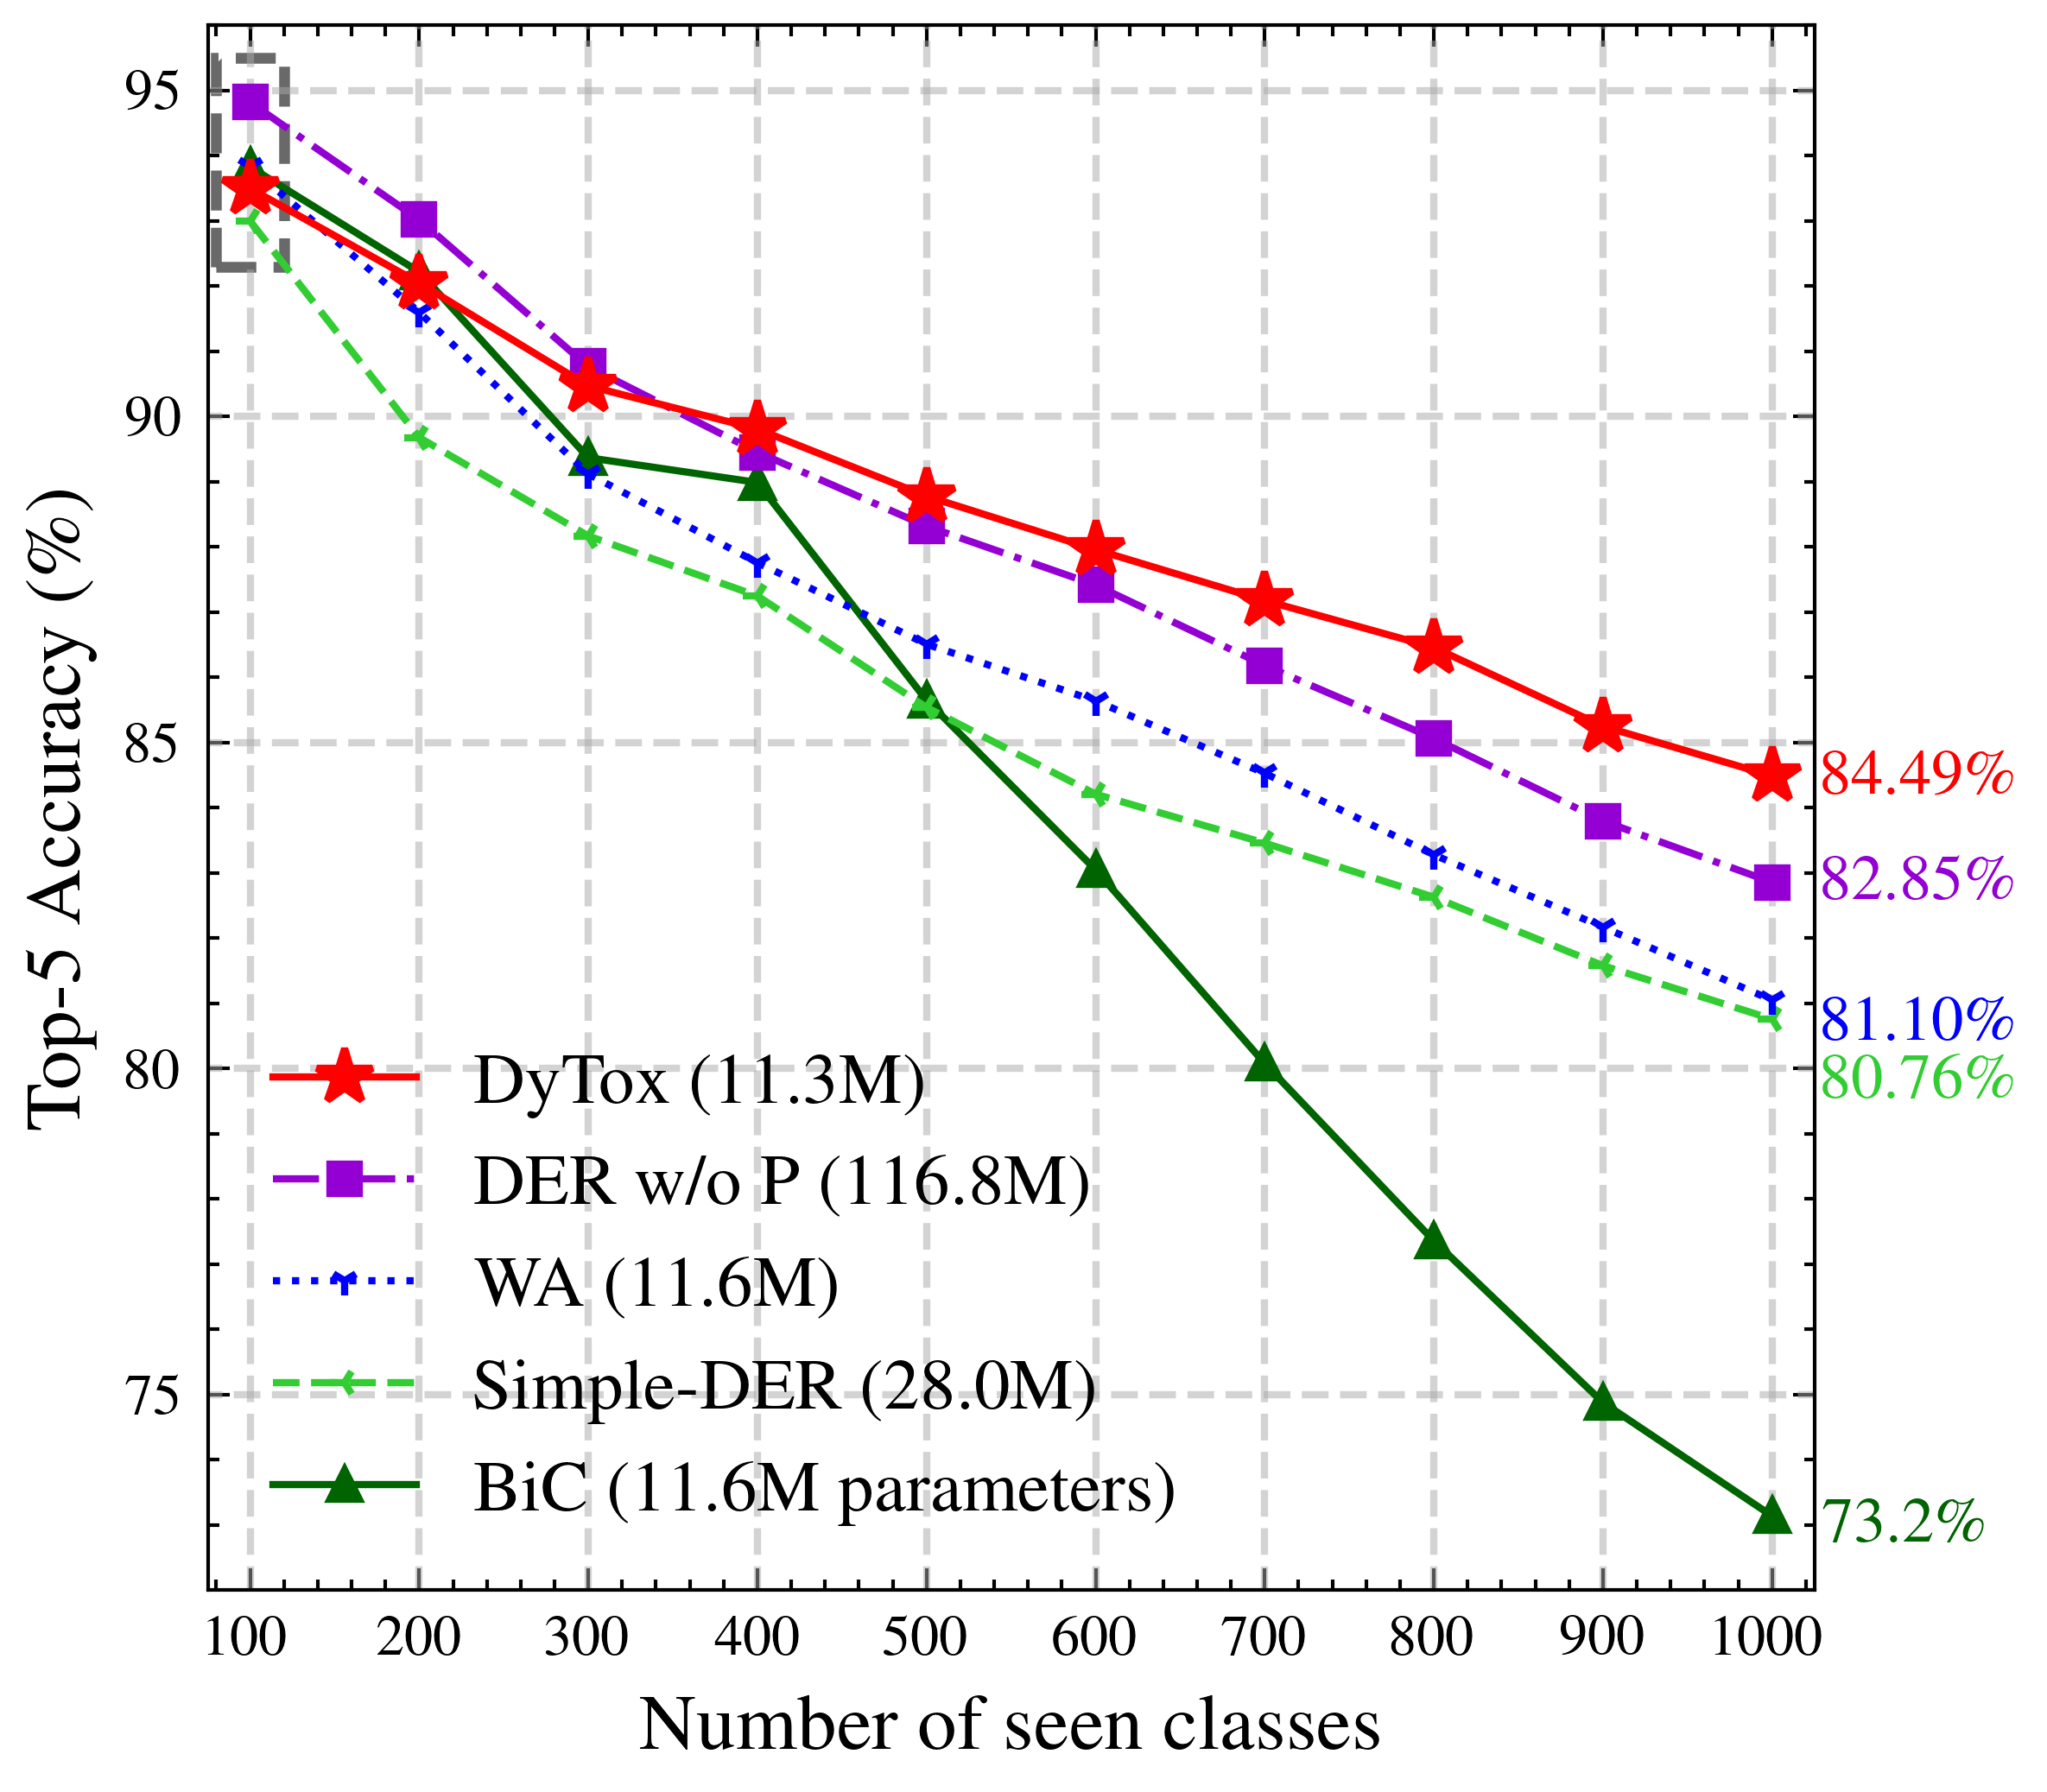
\includegraphics[width=0.9\textwidth]{images/dytox/imagenet1000.png}
        \caption{\textbf{ImageNet1000}}
        \label{fig:dytox_imagenet1000}
    \end{subfigure}%
    \begin{subfigure}{.5\textwidth}
        \centering
        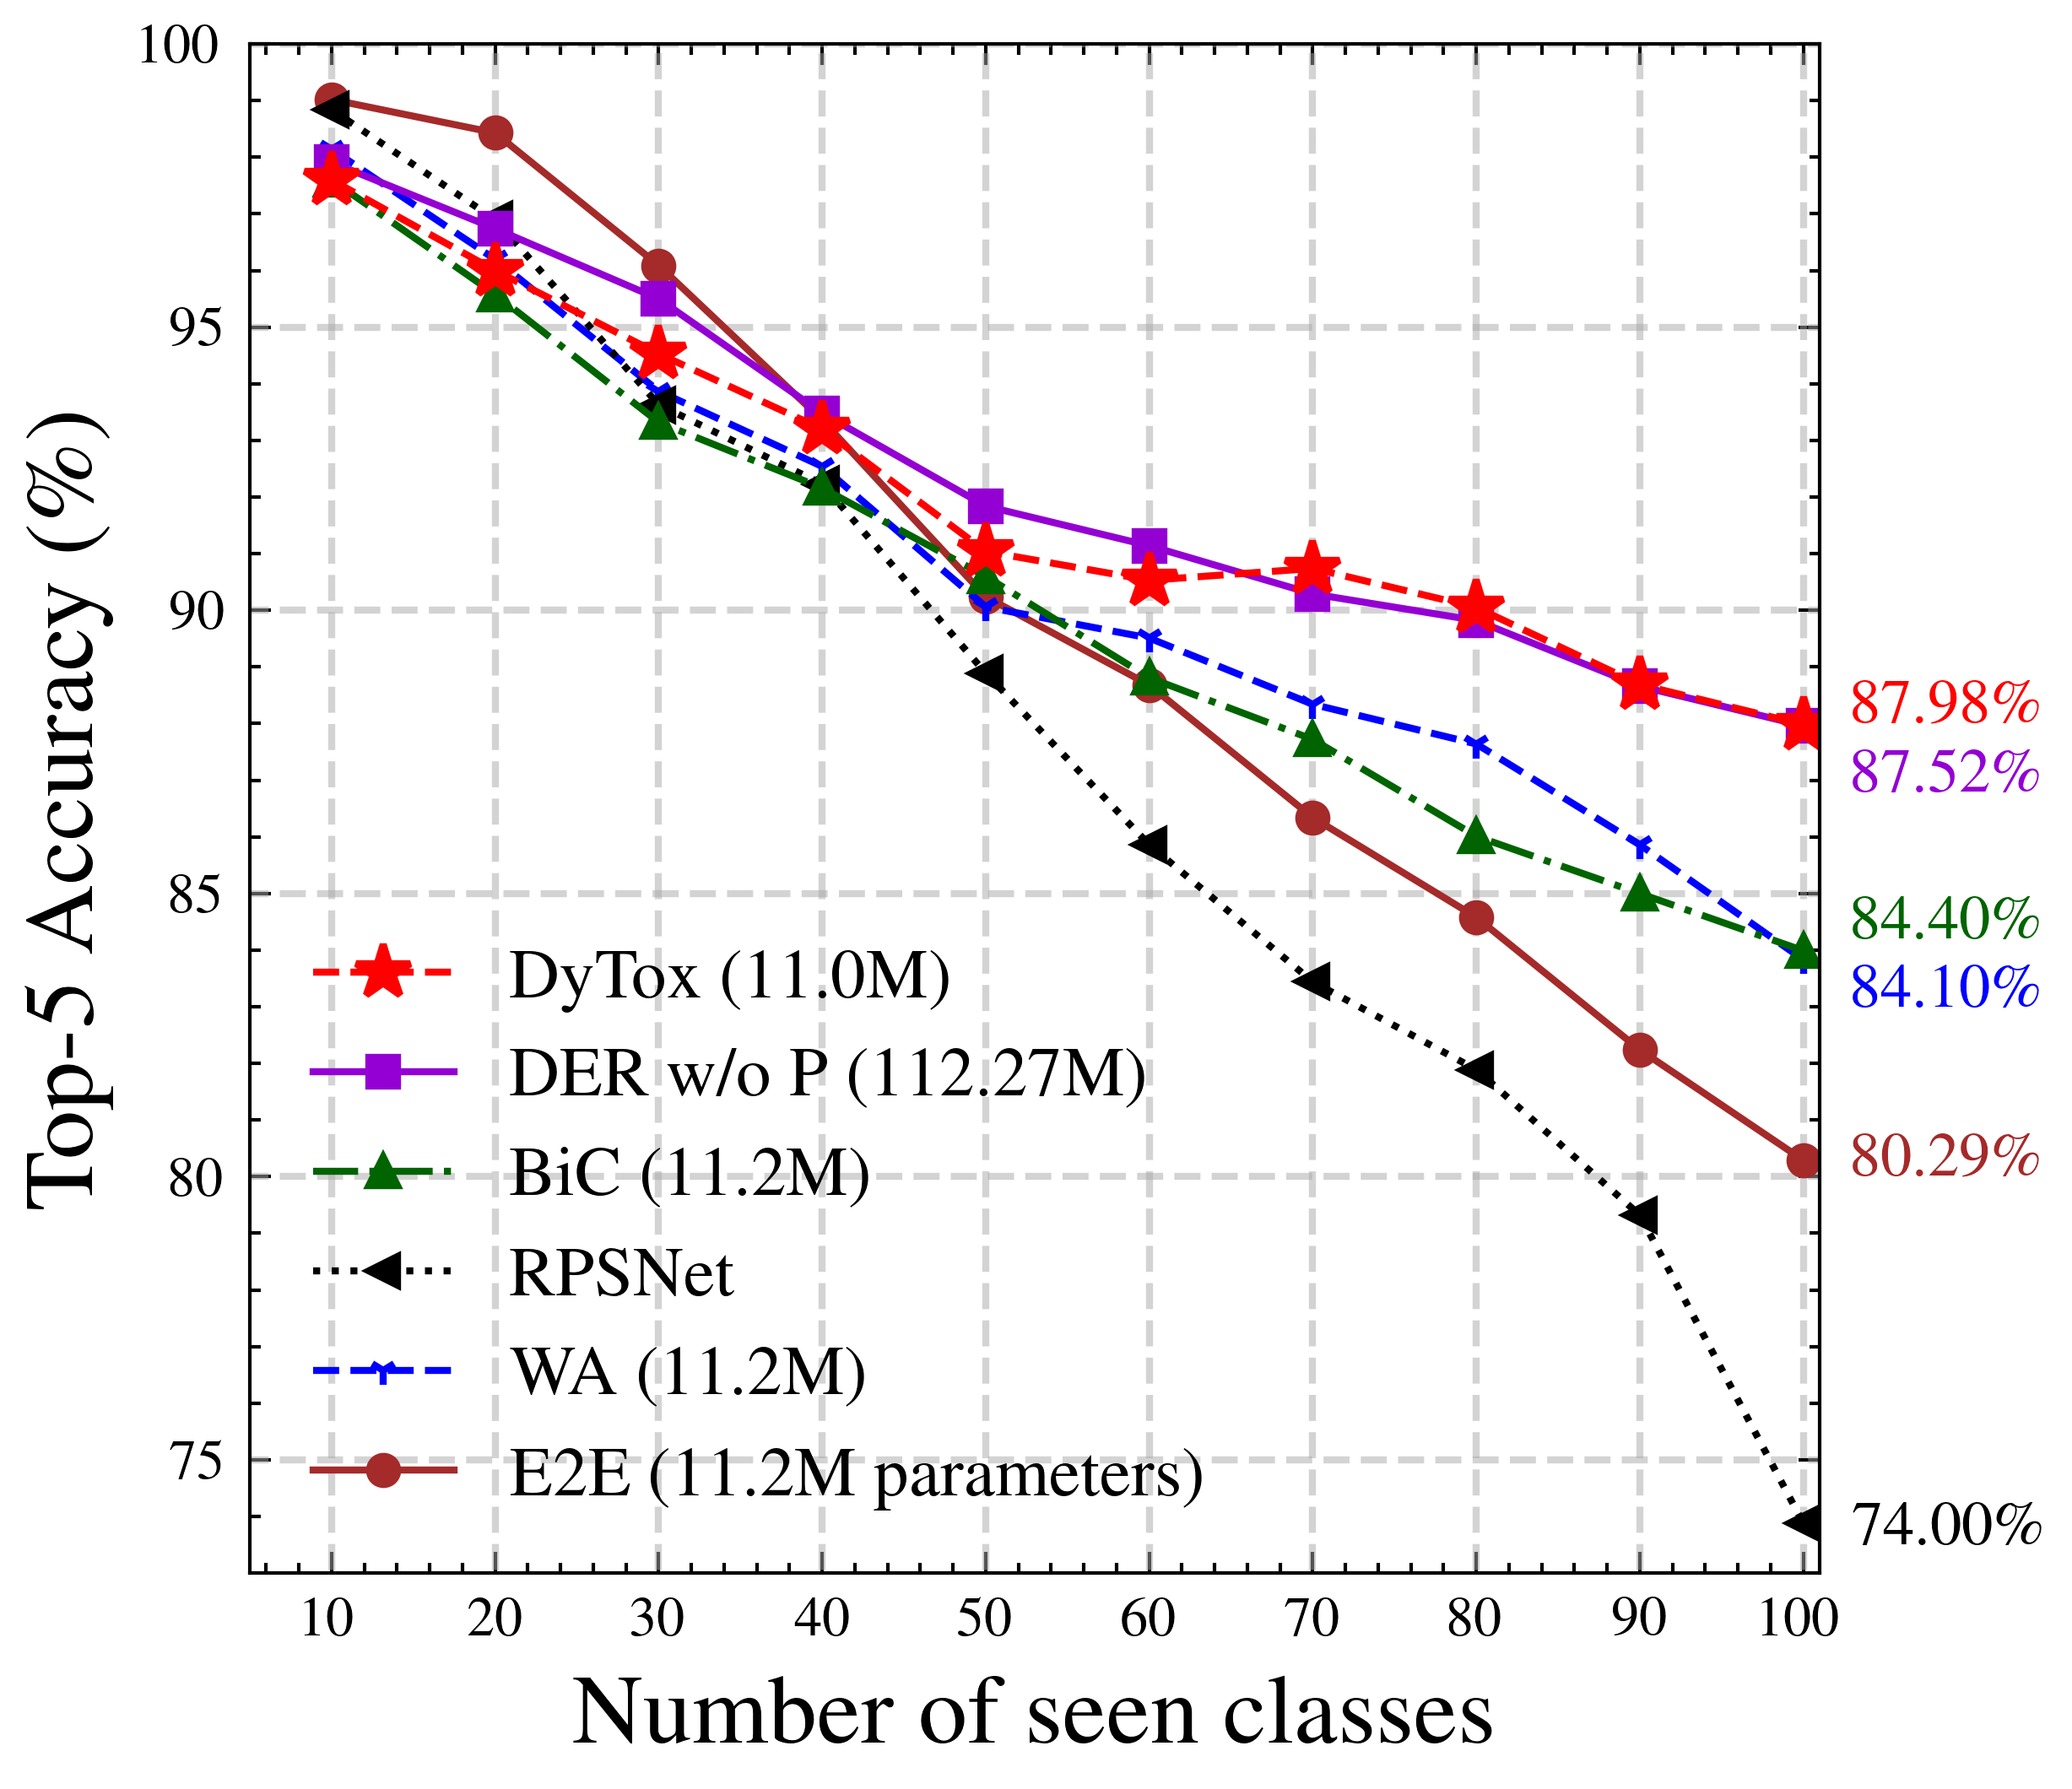
\includegraphics[width=0.9\textwidth]{images/dytox/imagenet100.png}
        \caption{\textbf{ImageNet100}}
        \label{fig:dytox_imagenet100}
    \end{subfigure}
    \caption{\textbf{Performance evolution on ImageNet-\{100, 1000\}.} The top-5 accuracy (\%) is
        reported after learning each task. Our model DyTox (in \textbf{\textcolor{red}{red}}) reaches
        state-of-the-art performance while using significantly fewer parameters than concurrent models.
        Note that at the initial step before the continual process begins, our model has performance
        comparable to other baselines: the performance gain is achieved by reducing catastrophic
        forgetting.}
    \label{fig:dytox_imagenet}
\end{figure}


\subsection{Quantitative results}

\paragraph{ImageNet}
We report performances in \autoref{tab:dytox_imagenet} and in \autoref{tab:dytox_imagenet_pp} for
respectively the ImageNet-1000 and ImageNet-100 dataset. The $^\dagger$
marks the DER with setting-specific pruning, and DER w/o P is for the DER without pruning.
Critically, on the larger-scale ImageNet1000, DyTox systematically performs best on all
metrics despite having lower parameters count. Specifically, DyTox reaches 71.29\% in ``Avg'' top-1
accuracy, and 63.34\% in ``Last'' top-1 accuracy. This outperforms the previous state-of-the-art DER
w/o P (68.84\% in ``Avg'', 60.16\% in ``Last'') which has 10 ResNet18 in parallel and 116.89M
parameters. Compared to the pruned DER$^\dagger$, DyTox has a +4.56 \pp in top-1 and a +1.51 \pp in
top-5 for the ``Avg'' accuracy. In ImageNet100, DyTox reaches 69.10\% and outperforms DER$^\dagger$ by +3.04 percentage points (\pp) in
``Last'' top-1 accuracy. Though, DyTox and DER w/o P somehow perform similarly in ``Avg'' accuracy,
DyTox+ and DyTox++ reach state-of-the-art performance. Specifically, DyTox++, using our full
improved continual training procedure, improves the ``Avg'' top-1 accuracy of DER by 3.58 \pp.

All models evolutions on ImageNet-1000 and ImageNet-100 are illustrated in
\autoref{fig:dytox_imagenet}: DyTox constantly surpasses previous state-of-the-art models --- despite
having a comparable performance at the first step and fewer parameters.

\begin{table*}[t]
    \centering
    \resizebox{1.0\textwidth}{!}{%
        \begin{tabular}{@{}l|ccc|ccc|ccc}
            \hline
                                                                     & \multicolumn{3}{c}{10 steps} & \multicolumn{3}{c}{20 steps}                  & \multicolumn{3}{c}{50 steps}                                                                                                                                                                                                                   \\
            \textbf{Methods}                                         & \textbf{\#P}                 & \textbf{Avg}                                  & \textbf{Last}                & \textbf{\#P}        & \textbf{Avg}                                  & \textbf{Last}                    & \textbf{\#P}        & \textbf{Avg}                                  & \textbf{Last}                    \\
            \hline
            ResNet18 Joint                                           & 11.22                        & -                                             & 80.41                        & 11.22               & -                                             & 81.49                            & 11.22               & -                                             & 81.74                            \\
            Transf. Joint                                            & 10.72                        & -                                             & 76.12                        & 10.72               & -                                             & 76.12                            & 10.72               & -                                             & 76.12                            \\
            \hline
            iCaRL \cite{rebuffi2017icarl}                            & 11.22                        & 65.27\scriptsize{\mypm1.02}                   & 50.74                        & 11.22               & 61.20\scriptsize{\mypm0.83}                   & 43.75                            & 11.22               & 56.08\scriptsize{\mypm0.83}                   & 36.62                            \\
            UCIR \cite{hou2019ucir}                                  & 11.22                        & 58.66\scriptsize{\mypm0.71}                   & 43.39                        & 11.22               & 58.17\scriptsize{\mypm0.30}                   & 40.63                            & 11.22               & 56.86\scriptsize{\mypm0.83}                   & 37.09                            \\
            BiC \cite{wu2019bias_correction}                         & 11.22                        & 68.80\scriptsize{\mypm1.20}                   & 53.54                        & 11.22               & 66.48\scriptsize{\mypm0.32}                   & 47.02                            & 11.22               & 62.09\scriptsize{\mypm0.85}                   & 41.04                            \\
            WA \cite{zhao2020weightalignement}                       & 11.22                        & 69.46\scriptsize{\mypm0.29}                   & 53.78                        & 11.22               & 67.33\scriptsize{\mypm0.15}                   & 47.31                            & 11.22               & 64.32\scriptsize{\mypm0.28}                   & 42.14                            \\
            PODNet \cite{douillard2020podnet}                        & 11.22                        & 58.03\scriptsize{\mypm1.27}                   & 41.05                        & 11.22               & 53.97\scriptsize{\mypm0.85}                   & 35.02                            & 11.22               & 51.19\scriptsize{\mypm1.02}                   & 32.99                            \\
            RPSNet \cite{rajasegaran2019rpsnet}                      & 56.5\,\,                     & 68.60                                         & 57.05                        & -                   & -                                             & -                                & -                   & -                                             & -                                \\
            DER \small{w/o P} \cite{yan2021der}                      & 112.27                       & 75.36\scriptsize{\mypm0.36}                   & \textbf{65.22}               & 224.55              & 74.09\scriptsize{\mypm0.33}                   & 62.48                            & 561.39              & 72.41\scriptsize{\mypm0.36}                   & 59.08                            \\ % no pruning
            \textcolor{gray}{$\text{DER}^\dagger$} \cite{yan2021der} & \textcolor{gray}{-}          & \textcolor{gray}{74.64\scriptsize{\mypm0.28}} & \textcolor{gray}{64.35}      & \textcolor{gray}{-} & \textcolor{gray}{73.98\scriptsize{\mypm0.36}} & \textcolor{gray}{\textbf{62.55}} & \textcolor{gray}{-} & \textcolor{gray}{72.05\scriptsize{\mypm0.55}} & \textcolor{gray}{\textbf{59.76}} \\
            \hline
            DyTox                                                    & 10.73                        & 73.66\mysmpm{0.02}                            & 60.67\mysmpm{0.34}           & 10.74               & 72.27\mysmpm{0.18}                            & 56.32\mysmpm{{0.61}}             & 10.77               & 70.20\mysmpm{0.16}                            & 52.34\mysmpm{0.26}               \\
            DyTox+                                                   & 10.73                        & \textbf{75.54}\mysmpm{0.10}                   & 62.06\mysmpm{0.25}           & 10.74               & \textbf{75.04}\mysmpm{0.11}                   & 60.03\mysmpm{0.45}               & 10.77               & \textbf{74.35}\mysmpm{0.05}                   & 57.09\mysmpm{0.13}               \\
            \hline
        \end{tabular}
    }
    \caption{\textbf{Results on CIFAR100} averaged over three different class orders. Baselines
        results are come from \cite{yan2021der}. The $\dagger$ symbol means that \cite{yan2021der}
        needed setting-sensitive hyperparameters. Moreover, its reported parameters count was an average
        over all steps: the final parameters count (necessarily higher) was not available.}
    \label{tab:dytox_cifar100-b0}
\end{table*}


\begin{figure*}[t!]
    \centering
    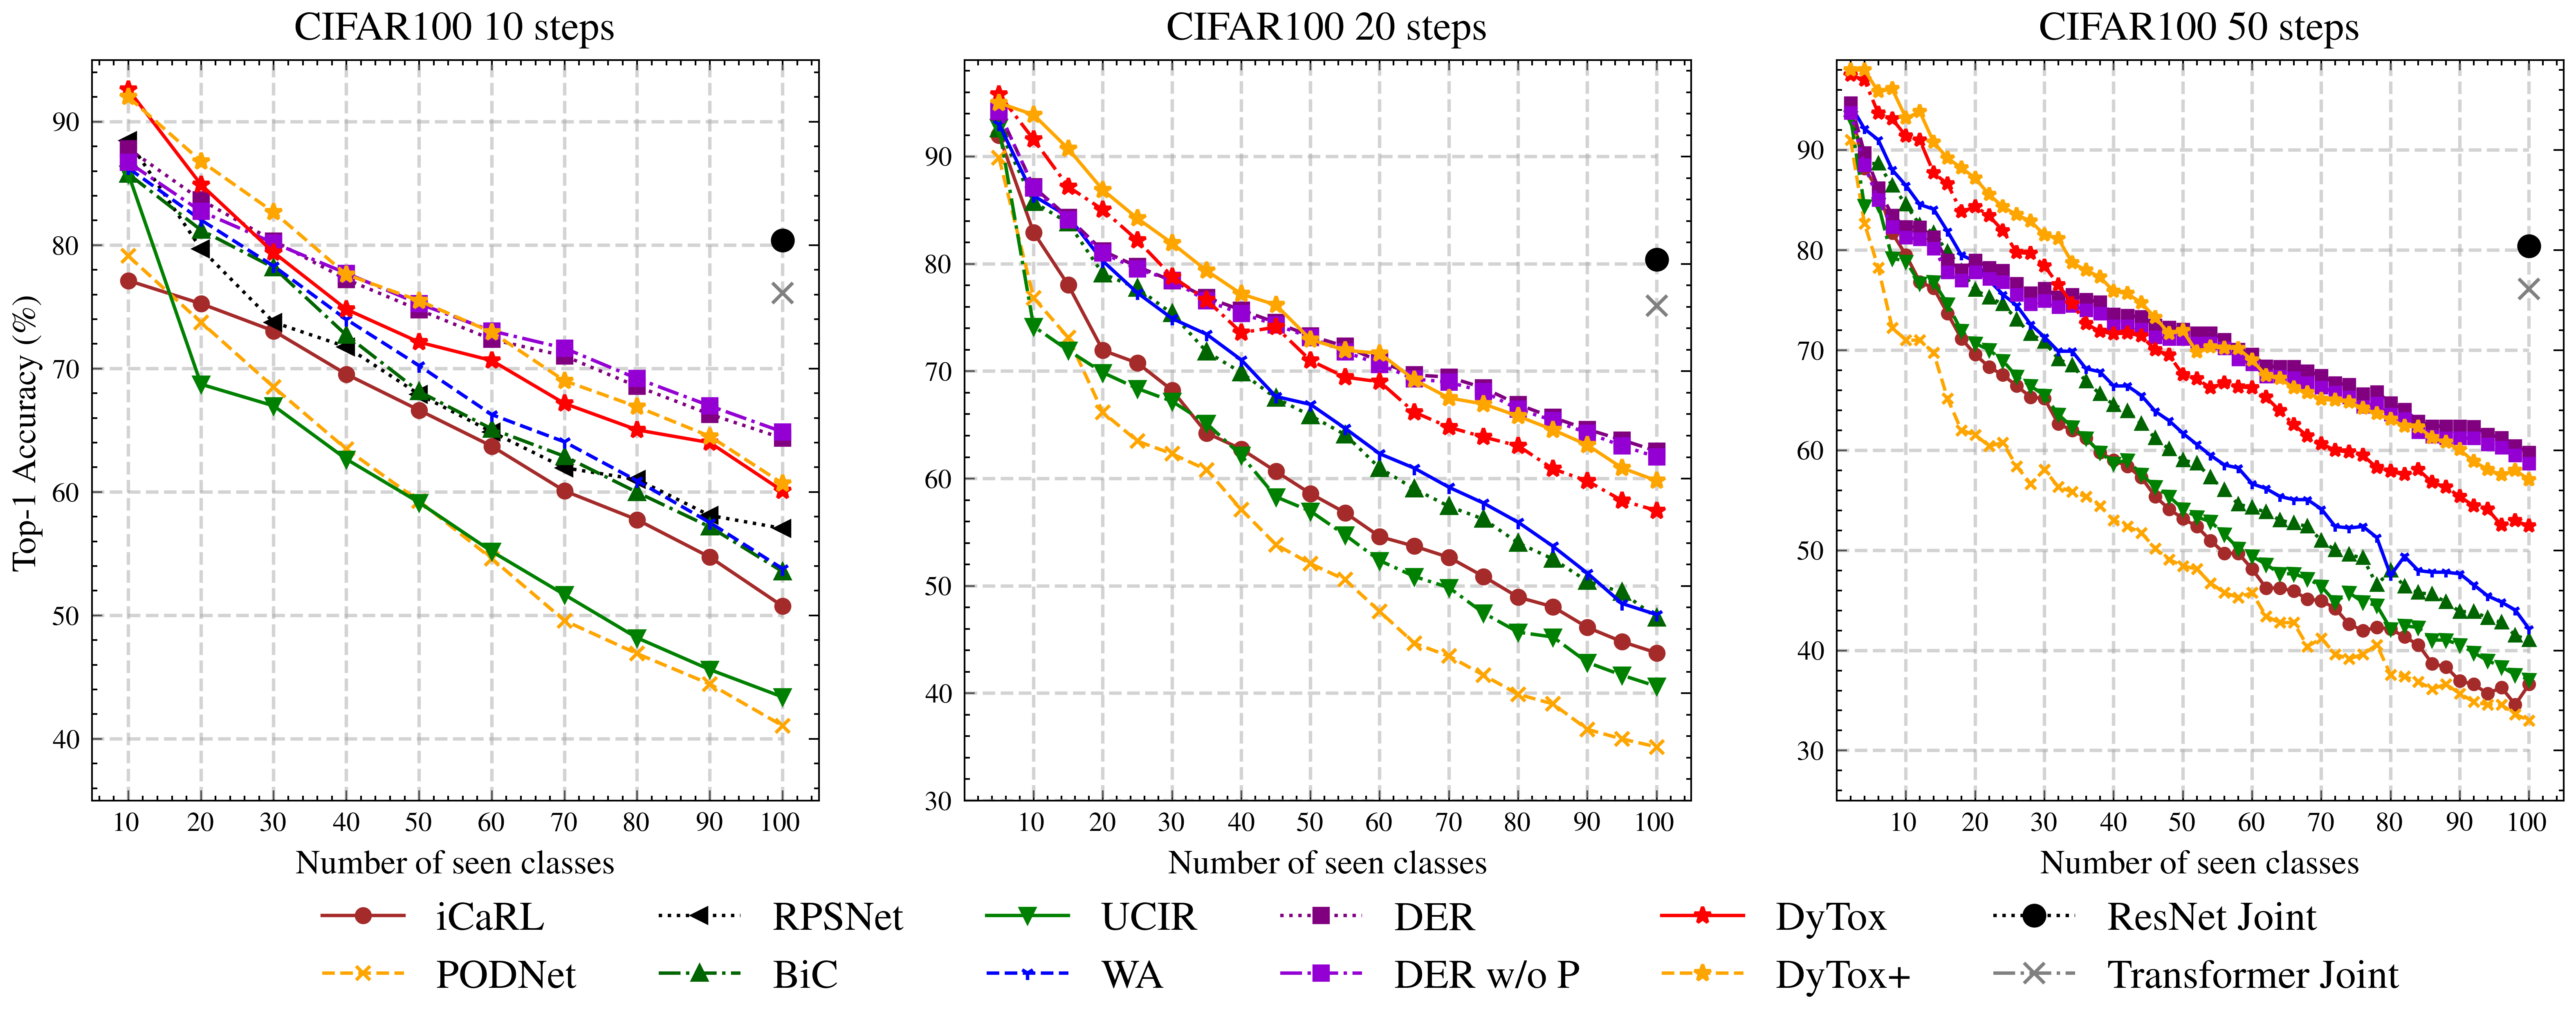
\includegraphics[width=1.0\linewidth]{images/dytox/cifar.png}
    \caption{\textbf{Performance evolution on CIFAR100}. The top-1 accuracy (\%) is reported after
        learning each task. \textbf{Left} is evaluated with 10 steps, \textbf{middle} with 20 steps, and
        \textbf{right} with 50 steps.}
    \label{fig:dytox_increment_cifar}
\end{figure*}

DyTox is able to scale correctly while handling seamlessly the parameter growth by sharing most of
the weights across tasks. In contrast, DER had to propose a complex pruning method; unfortunately,
this pruning required different hyperparameter values for different settings. Despite this, the
pruning in DER$^\dagger$ is less efficient when classes diversity increase: DER$^\dagger$ doubles in
size between ImageNet100 and ImageNet1000 (\citet{yan2021der} report 7.67M \textit{vs.} 14.52M)
while handling the same amount of tasks (10). Note that these parameter counts reported for
DER$^\dagger$ in \citet{yan2021der} are in fact averages over all steps: the final parameters count
(necessarily higher) was not available and thus is not reported in our tables. Simple-DER also
applies pruning but without hyperparameter tuning; while simpler, the pruning is also less efficient
and induces larger model (28.00M parameters).

%\vspace{-0.5em}
\paragraph{CIFAR100} \autoref{tab:dytox_cifar100-b0} shows results for all approaches on CIFAR100.
The more steps there are, the larger the forgetting is and thus the lower the performances are.
Those settings are also displayed in \autoref{fig:dytox_increment_cifar} after each task. In every
setting, DyTox is close to DER w/o P  for much fewer parameters (up to 52x less). Critically, DyTox
is significantly above other baselines: \eg DyTox is up to +25\% in ``Last'' accuracy in the 50
steps setup. Note that our improved continual training procedure, with DyTox+ and DyToX++, further
increases the results in all settings. Notably DyTox++ increases the ``Àvg'' accuracy in the 50
setup over DER by +3.4 \pp. Remark also that DER ``Avg'' accuracy degrades by 2.59 \pp between the
easiest 10 steps setting and the hardest 50 steps setting. In comparison, DyTox++ only loses 1.65
\pp, proving a better robustness to forgetting as the number of tasks increases. Remark that the
results in this table of our PODNet, presented in \autoref{chapter:regularization}, can be explained
because of the slightly different setting: PODNet was designed for situation where half of the
dataset's classes were learned in a single step, and thus providing a better initialization. PODNet,
a metric-based model (as also UCIR), excelled in those situations, but struggle when the initial
step contains few classes (as it is the case in this chapter) due to slower initial learning.
Arguably, in a real-life scenario, a model should be pretrained on a large dataset and therefore
this ``\textit{weakness}'' of PODNet won't materialize.

\subsection{Model introspection on CIFAR100}

\paragraph{Memory overhead}
We only add a vector of size $d=384$ per task; thus, the overhead in memory (not considering the
growing classifier which is common for all continual models) is only of $+0.004\%$ per step. Even in
the challenging setting of CIFAR100 with 50 tasks, our memory overhead is almost null ($+0.2\%$).

\label{sec:dytox_comp_over}
%\vspace{-1em}
\paragraph{Computational overhead} The vast majority of the computation is done in the SABs, thus
shared among all tasks. The dynamical component of our model is located at the ultimate TAB.
Moreover, the Task-Attention, contrary to the Self-Attention, has a time complexity linear in terms
of tokens and not quadratic reducing the time overhead to an acceptable sub-linear amount. Overall,
for each new task, one forward pass is only $2.24\%$ slower than at the previous task.
Furthermore, the procedure can be accelerated by doing a single forward pass through the TAB with
a masked attention \citep{vaswani2017transformer}: the query is the concatenation of all task
tokens, then we mask the attention logits corresponding to an interaction between task tokens. For
an almost equivalent result (modulo numerical imprecision), a new task only increases the time spent
in a forward pass by $1.09\%$.

%\vspace{-1em}
\begin{table}[t]
    \centering
    \begin{tabular}{@{}l|c|ccc}
        \hline
                          & Joint (1 step)                                  & \multicolumn{2}{c}{50 steps}                                                                             \\
        \textbf{Training} & \textbf{Last} ($\uparrow$)                      & \textbf{Last} ($\uparrow$)                      & \textbf{Forgetting} ($\downarrow$)\Tstrut\Bstrut       \\
        \hline
        DyTox             & 76.12                                           & 52.34                                           & 33.15 \Tstrut                                          \\
        DyTox+            & 77.51\scriptsize{\textcolor{OliveGreen}{+1.39}} & 57.09\scriptsize{\textcolor{OliveGreen}{+4.75}} & 31.50\scriptsize{\textcolor{OliveGreen}{-1.65}}\Bstrut \\
        DyTox++           & 77.91\scriptsize{\textcolor{OliveGreen}{+0.40}} & 58.76\scriptsize{\textcolor{OliveGreen}{+1.67}} & 30.47\scriptsize{\textcolor{OliveGreen}{-1.03}}        \\
        \hline
    \end{tabular}
    \caption{\textbf{``Last'' accuracy and forgetting} \cite{chaudhry2018riemannien_walk} on
        CIFAR100 for the joint (1 step, no continual) and 50 steps settings.}
    \label{tab:dytox_training_plus}
\end{table}


\paragraph{Training procedure introspection} Our DyTox+ and DyTox++ strategies really reduce
catastrophic forgetting and does not just improve raw performances. This is shown in
\autoref{tab:dytox_training_plusplus}, where we compare DyTox \vs DyTox+ \vs DyTox++ strategies on
CIFAR100. In the joint setting, our model slightly benefits from both MixUp and ASAM: the gain is
limited (+1.79 \pp). On the other hand, those two methods greatly improve the extreme
continual setting of 50 steps (+6.42 \pp). This shows that the gain is not due to absolute
improvements of the model performance. Moreover, using the forgetting measure of
\citet{chaudhry2018riemannien_walk}, we compare how much a model has forgotten relatively to its
previous tasks. This metric is therefore agnostic to absolute performance improvements. DyTox had a
forgetting of 33.15\%, DyTox+ of 31.50\%, and DyTox++ of 30.47\%: a total reduction of 2.68 \pp.
This validates our novel training procedures that are particularly efficient for continual learning.
The computational overhead of ASAM is lower than more complex second-order methods, but it still
doubles the number of forward and backward passes. For this reason, we didn't evaluated DyTox++ on
the large ImageNet1000. However, future works could consider the promising Look-SAM
\cite{liu2021looksam} to reduce the time overhead.

\begin{table}
    \centering
    \begin{tabular}{ll|ccccc|cc}
         &                                                                                               & \rot{\footnotesize{Knowledge Distillation}} & \rot{\footnotesize{Finetuning}} & \rot{\footnotesize{Token Expansion}} & \rot{\footnotesize{Divergence Classifier}} & \rot{\footnotesize{Indendepent Classifiers}} & \textbf{Avg} & \textbf{Last} \\
        \hline
        \parbox[t]{2mm}{\multirow{7}{*}{\rotatebox[origin=c]{90}{\textbf{DyTox}}}}
         & \parbox[t]{3mm}{\multirow{3}{*}{\rotatebox[origin=c]{90}{\textbf{\scriptsize{Transformer}}}}}
         &                                                                                               &                                             &                                 &                                      &                                            & 60.69                                        & 38.87\Tstrut                 \\
         &                                                                                               & \cmark                                      &                                 &                                      &                                            &                                              & 61.62        & 39.35         \\
         &                                                                                               & \cmark                                      & \cmark                          &                                      &                                            &                                              & 63.42        & 42.21         \\[3pt]
        %\vspace{0.01cm}
        \cline{2-9}
         & \parbox[t]{3mm}{\multirow{3}{*}{\rotatebox[origin=c]{90}{\textbf{\scriptsize{Dynamic}}}}}
         & \cmark                                                                                        & \cmark                                      & \cmark                          &                                      &                                            & 67.30                                        & 47.57\Tstrut                 \\
         &                                                                                               & \cmark                                      & \cmark                          & \cmark                               & \cmark                                     &                                              & 68.28        & 49.45         \\
         &                                                                                               & \cmark                                      & \cmark                          & \cmark                               & \cmark                                     & \cmark                                       & 70.20        & 52.34\Bstrut  \\
        \hline
    \end{tabular}
    \caption{\textbf{Ablations} of the different key components of our DyTox architecture. We report
    the average accuracy and the last accuracy on CIFAR100 for the setting with 50
    steps.\vspace{-1em}}
    \label{tab:dytox_ablation}
\end{table}

\FloatBarrier

%\vspace{-1em}
\label{sec:dytox_ablations}
\paragraph{Model ablations} We ablate the importance of the different components of DyTox in
\autoref{tab:dytox_ablation}. We add on the base transformer a naive knowledge distillation
\citep{hinton2015knowledge_distillation} and a finetuning
\citep{castro2018end_to_end_inc_learn} applied after each
task on a balanced set of new data and rehearsal data. Finally, our DyTox strategy exploits directly
the very nature of transformers (separated task information from the pixels information) to tackle
catastrophic forgetting with three components: (1) a task token expansion, (2) a divergence
classifier, and (3) independent classifiers. All three greatly improve over the baseline transformer
($42.21\% \rightarrow 52.34\%$ in ``Last'') while having almost no memory overhead ($+0.2\%$). The
divergence classifier improves the diversity between task tokens: we observed that the minimal
Euclidean distance between them increases by 8\%. Moreover, we also remarked that having independent
classifiers reduces the forgetting defined by \citet{chaudhry2018riemannien_walk} by more than
24\%.


\section{Conclusion}

In this chapter, we covered our work on dynamic architectures. While in previous chapters, we aimed
to constrain the visual features, we decided here to condition the features to specific tasks. With
DyTox, a new dynamic strategy for continual learning based on transformer architecture, all tasks
share a common encoding produced by self-attention layers. Then, task-specific tokens are used to
produce task-specialized embeddings through a new task-attention layer. This architecture allows
to dynamically process new tasks with very little memory overhead and does not require complex
hyperparameter tuning. Our experiments show that our framework scales to large datasets and an
important number of tasks efficiently while using significantly fewer parameters than concurrent
dynamic strategies.
